\documentclass{standalone}
\usepackage{tikz}
\usetikzlibrary{shapes,arrows.meta}
\begin{document}
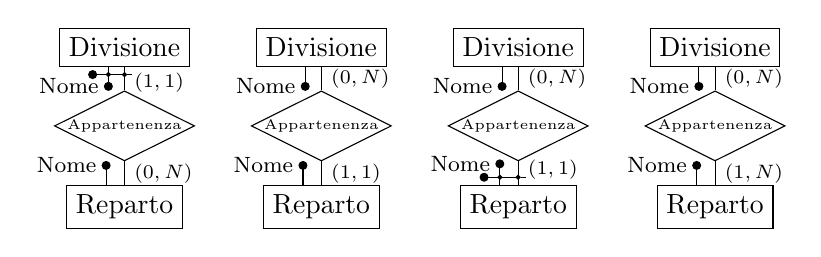
\begin{tikzpicture}
    \draw

    %%* Attributi:
    %%  node[draw, circle, inner sep=1pt, fill=black]{}node[right]{\footnotesize A}
    %%? Distanza orizzontale: E -(0.25,0.x)- A
    %%? Distanza verticale: E -(0,x * 0.22)- A

    %%* Cardinalità:
    %%  node[below right]{\scriptsize $(0,N)$}
    %%  node[above right]{\scriptsize $(0,N)$}
    %%  node[midway, above]{\scriptsize $(0,N)$}

    %%* Relazione:
    %%  node[draw, diamond, shape aspect=2, inner sep=3pt, anchor=90](r1){}
    %%  node[draw, diamond, shape aspect=2, inner sep=0.2pt, anchor=180](r2){R2}

    %%* Entità:
    %%  node[draw, rectangle, anchor=90](e1){}
    %%? Distanza verticale: E -(0.3)- R -(0.3) E
    %%? Distanza orizzontale: E -(0.75)- R -(0.75)- E

    %%* Schema 1
    (0,0)node[draw, rectangle, anchor=90](e1){Divisione}
    (e1.230)--++(0,-0.1)node[draw, circle, inner sep=0.5pt, fill=black](a){}--++(0,-0.15)node[draw, circle, inner sep=1pt, fill=black]{}node[left]{\footnotesize Nome}
    (e1.270)--++(0,-0.1)node[draw, circle, inner sep=0.5pt, fill=black](b){}--++(0,-0.2)node[midway, right]{\scriptsize $(1,1)$}node[draw, diamond, shape aspect=2, inner sep=0.1pt, anchor=90](r1){\tiny Appartenenza}
    (r1.270)--++(0,-0.3)node[midway, right]{\scriptsize $(0,N)$}node[draw, rectangle, anchor=90](r){Reparto}
    (r.130)--++(0,0.25)node[draw, circle, inner sep=1pt, fill=black]{}node[left]{\footnotesize Nome}
    (a)++(-0.2,0)node[draw, circle, inner sep=1pt, fill=black]{}--(b)--++(0.1,0)

    %%* Schema 2
    (2.5,0)node[draw, rectangle, anchor=90](e1){Divisione}
    (e1.230)--++(0,-0.25)node[draw, circle, inner sep=1pt, fill=black]{}node[left]{\footnotesize Nome}
    (e1.270)--++(0,-0.3)node[midway, right]{\scriptsize $(0,N)$}node[draw, diamond, shape aspect=2, inner sep=0.1pt, anchor=90](r1){\tiny Appartenenza}
    (r1.270)--++(0,-0.3)node[midway, right]{\scriptsize $(1,1)$}node[draw, rectangle, anchor=90](r){Reparto}
    (r.130)--++(0,0.25)node[draw, circle, inner sep=1pt, fill=black]{}node[left]{\footnotesize Nome}


    %%* Schema 3
    (5,0)node[draw, rectangle, anchor=90](e1){Divisione}
    (e1.230)--++(0,-0.25)node[draw, circle, inner sep=1pt, fill=black]{}node[left]{\footnotesize Nome}
    (e1.270)--++(0,-0.3)node[midway, right]{\scriptsize $(0,N)$}node[draw, diamond, shape aspect=2, inner sep=0.1pt, anchor=90](r1){\tiny Appartenenza}
    (r1.270)--++(0,-0.2)node[midway, right]{\scriptsize $(1,1)$}node[draw, circle, inner sep=0.5pt, fill=black](b){}--++(0,-0.1)node[draw, rectangle, anchor=90](r){Reparto}
    (r.130)--++(0,0.1)node[draw, circle, inner sep=0.5pt, fill=black](a){}--++(0,0.17)node[draw, circle, inner sep=1pt, fill=black]{}node[left]{\footnotesize Nome}
    (a)++(-0.2,0)node[draw, circle, inner sep=1pt, fill=black]{}--(b)--++(0.1,0)


    %%* Schema 4
    (7.5,0)node[draw, rectangle, anchor=90](e1){Divisione}
    (e1.230)--++(0,-0.25)node[draw, circle, inner sep=1pt, fill=black]{}node[left]{\footnotesize Nome}
    (e1.270)--++(0,-0.3)node[midway, right]{\scriptsize $(0,N)$}node[draw, diamond, shape aspect=2, inner sep=0.1pt, anchor=90](r1){\tiny Appartenenza}
    (r1.270)--++(0,-0.3)node[midway, right]{\scriptsize $(1,N)$}node[draw, rectangle, anchor=90](r){Reparto}
    (r.130)--++(0,0.25)node[draw, circle, inner sep=1pt, fill=black]{}node[left]{\footnotesize Nome}
    ;
\end{tikzpicture}
\end{document}